\qrchapter{https://forgottenpillar.com/rsc/en-fp-chapter4}{Revision of “Living Temple”}


\qrchapter{https://forgottenpillar.com/rsc/en-fp-chapter4}{مراجعة “ليفينغ تمبل”}


In \textit{Testimonies for the Church Containing Letters to Physicians and Ministers Instruction to Seventh-Day Adventists}, the tenth chapter, \textit{The Foundation of our Faith,} God gave valuable lessons on the development and consequences of Kellogg's theories. The broader and deeper meaning of these quotations can be understood when we are familiar with their historical context. Let us first take a brief look at the historical context of Kellogg's book, The \textit{Living Temple}.


في \textit{تستومنيز فور ذا شرش كنتاينينغ لترز تو فيزيشنز أند منسترز انستركشن تو سفنث داي أدفنتستس}، الفصل العاشر، \textit{أساس إيماننا،} قدم الله دروسًا قيمة حول تطور وعواقب نظريات كيلوغ. يمكن فهم المعنى الأوسع والأعمق لهذه الاقتباسات عندما نكون على دراية بسياقها التاريخي. دعونا أولاً نلقي نظرة موجزة على السياق التاريخي لكتاب كيلوغ، \textit{ذا ليفينغ تمبل}.


In a series of providence, God signified that “\textit{Living Temple}” should not be printed. One such event was the burning of Battle Creek's press building, just the night before it was to be printed. Finally, the book was printed elsewhere; it instigated a great crisis in the Seventh-day Adventist Church. On October 7, 1903, a annual meeting of the conference was held in Washington DC. Many Seventh-day Adventist church leaders were present, including Dr. Kellogg and his sympathizers. Major controversy was taking place over this book and the conflict was inevitable. Fortunately, on the brink of this escalating conflict, a letter from Sister White was delivered to the council. On Sunday, the letter fell upon the ears of all, to which there resounded many “amen's” and “halleluyah's”. It was a very tense and moving morning for the church that was on the verge of a split—to at last have concrete direction from the Lord's messenger:


في سلسلة من العناية الإلهية، أشار الله إلى أن “\textit{ذا ليفينغ تمبل}” لا ينبغي أن يُطبع. أحد هذه الأحداث كان احتراق مبنى مطبعة باتل كريك، في الليلة التي سبقت طباعته. وأخيرًا، تمت طباعة الكتاب في مكان آخر؛ مما أثار أزمة كبيرة في كنيسة الأدفنتست السبتيين. في 7 أكتوبر 1903، عُقد اجتماع سنوي للمؤتمر في واشنطن العاصمة. كان العديد من قادة كنيسة الأدفنتست السبتيين حاضرين، بما في ذلك الدكتور كيلوغ والمتعاطفين معه. كان هناك جدل كبير يدور حول هذا الكتاب وكان الصراع أمرًا لا مفر منه. لحسن الحظ، على حافة هذا الصراع المتصاعد، تم تسليم رسالة من الأخت وايت إلى المجلس. يوم الأحد، وقعت الرسالة على آذان الجميع، وتردد صدى العديد من “آمين” و”هللويا”. كان صباحًا متوترًا ومؤثرًا للغاية بالنسبة للكنيسة التي كانت على وشك الانقسام - لتحصل أخيرًا على توجيه ملموس من رسول الرب:


\begin{figure}[h]
    \centering
    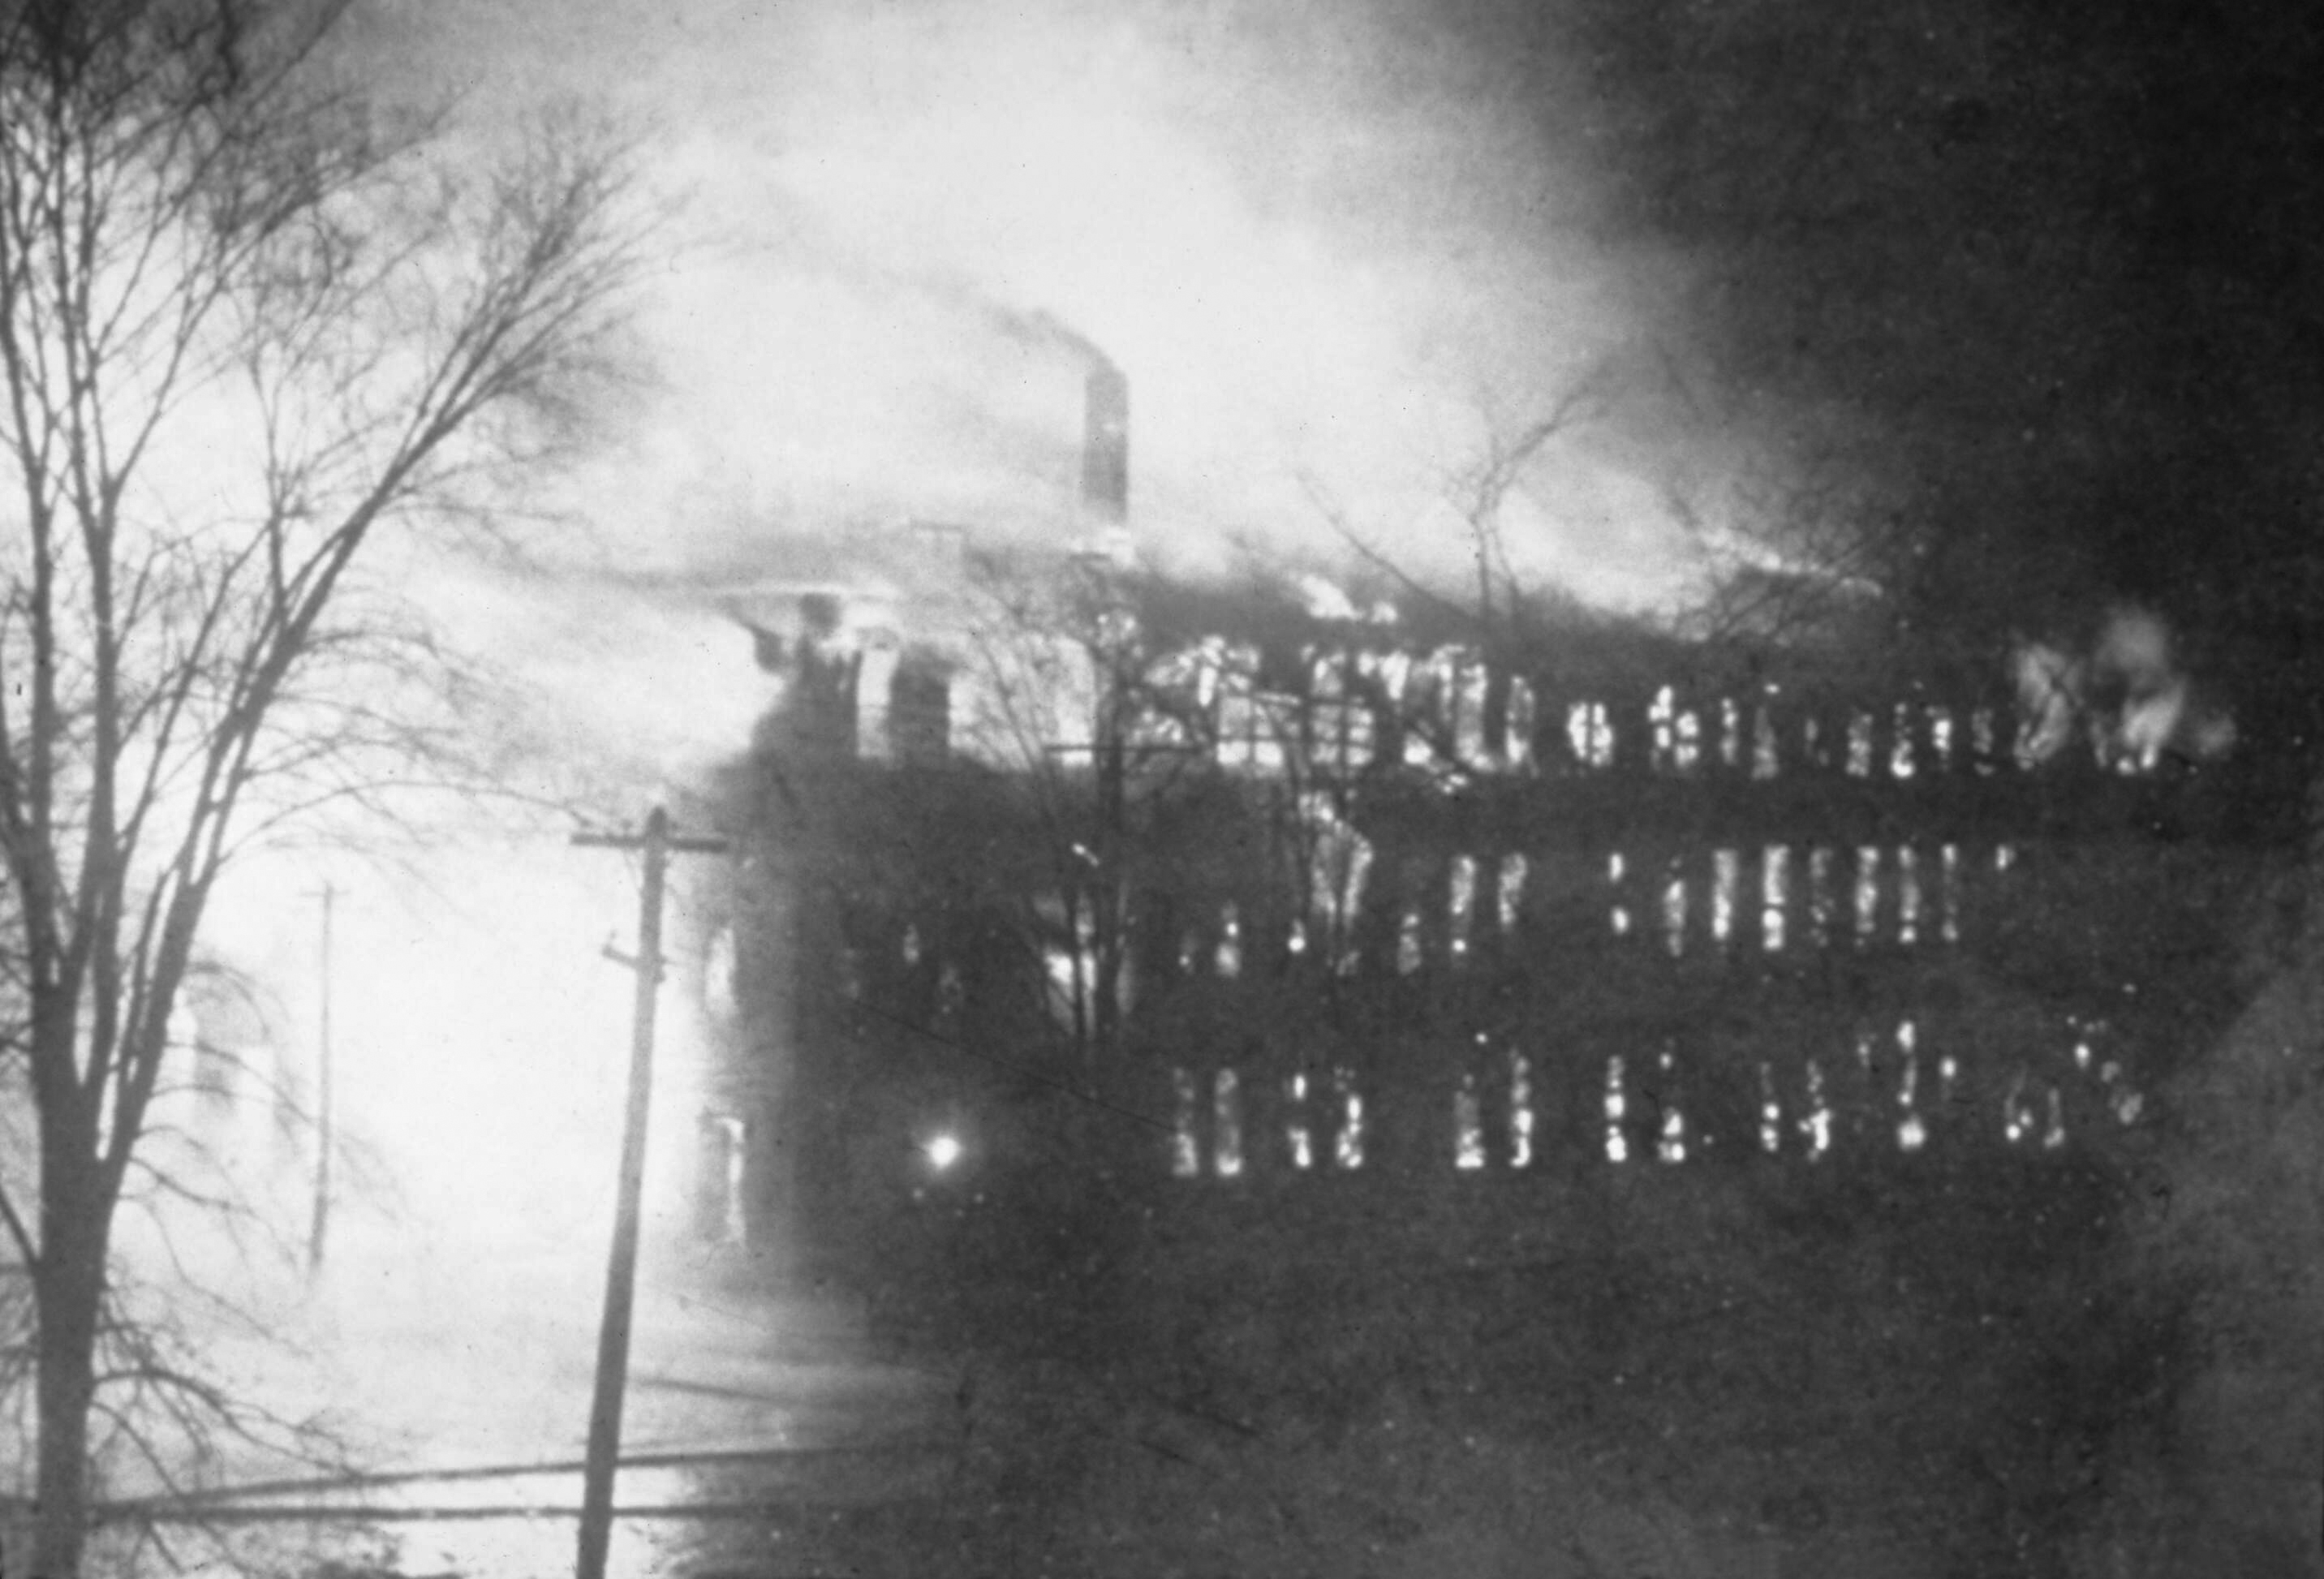
\includegraphics[width=1\linewidth]{images/review-and-herlad.jpg}
    \caption*{Burning of Review and Herald press building, December 30, 1902.}
    \label{fig:review-and-herald}
\end{figure}


\begin{figure}[h]
    \centering
    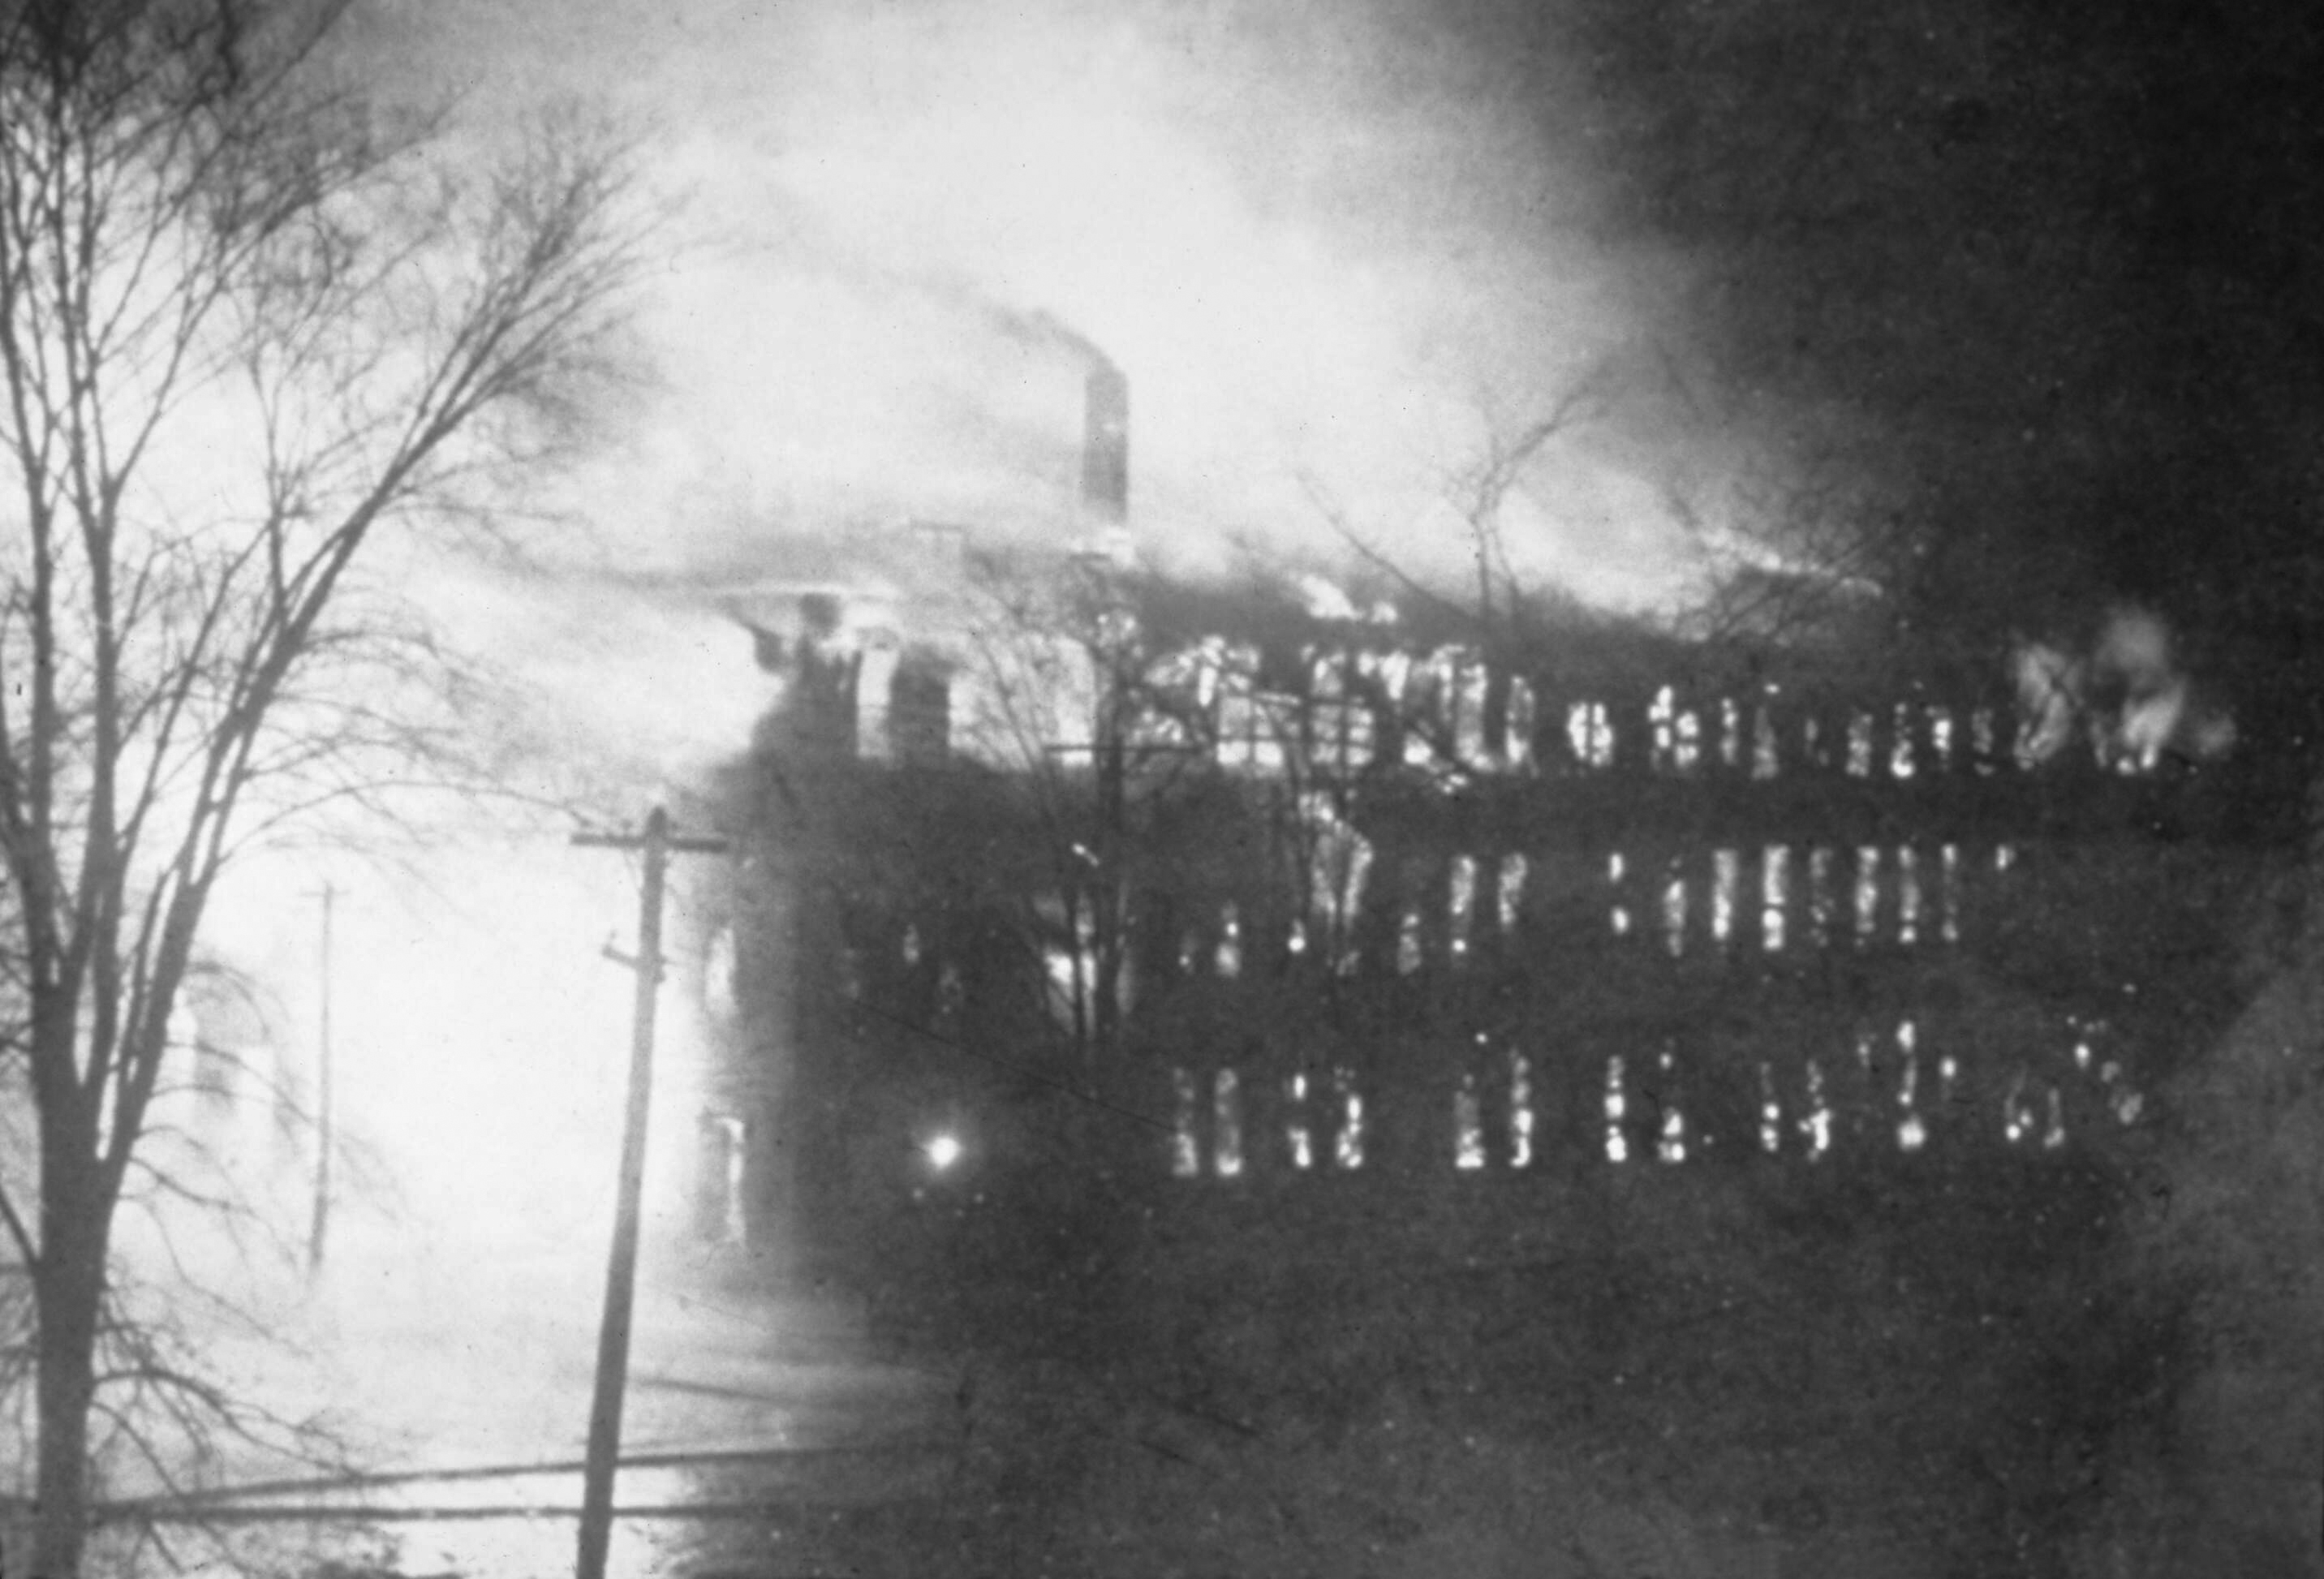
\includegraphics[width=1\linewidth]{images/review-and-herlad.jpg}
    \caption*{احتراق مبنى مطبعة ريفيو آند هيرالد، 30 ديسمبر 1902.}
    \label{fig:review-and-herald}
\end{figure}


\egw{I have some things to say to our teachers in reference to \textbf{the new book The Living Temple}. \textbf{Be careful how you sustain \underline{the sentiments of this book regarding the personality of God}}. As the Lord presents matters to me, \textbf{these sentiments do not bear the endorsement of God}. \textbf{They are a snare that the enemy has prepared for these last days}. I thought that this would surely be discerned and that it would not be necessary for me to say anything about it. \textbf{But since the claim has been made that the teachings of this book can be sustained by statements from my writings, I am compelled to speak in denial of this claim}. There may be in this book expressions and sentiments that are in harmony with my writings. And there may be in my writings many statements which when taken from their connection, and interpreted according to the mind of the writer of Living Temple, would seem to be in harmony with the teachings of this book. \textbf{This may give apparent support to the assertion that the sentiments in Living Temple are in harmony with my writings}. \textbf{But God forbid that this opinion should prevail}.}[Lt211-1903.1; 1903][https://egwwritings.org/read?panels=p14068.9598008]


\egw{لدي بعض الأشياء لأقولها لمعلمينا فيما يتعلق \textbf{بالكتاب الجديد ذا ليفينغ تمبل}. \textbf{كونوا حذرين في كيفية دعمكم \underline{للآراء الواردة في هذا الكتاب بخصوص شخصانية الله}}. كما يقدم الرب الأمور لي، \textbf{فإن هذه الآراء لا تحمل تأييد الله}. \textbf{إنها فخ أعده العدو لهذه الأيام الأخيرة}. ظننت أن هذا سيُدرك بالتأكيد وأنه لن يكون من الضروري أن أقول أي شيء عنه. \textbf{لكن بما أنه تم الادعاء بأن تعاليم هذا الكتاب يمكن دعمها بعبارات من كتاباتي، فأنا مضطرة للتحدث لإنكار هذا الادعاء}. قد تكون في هذا الكتاب تعبيرات وآراء متوافقة مع كتاباتي. وقد تكون في كتاباتي العديد من العبارات التي عندما تؤخذ خارج سياقها، وتُفسر وفقًا لعقل كاتب ذا ليفينغ تمبل، قد تبدو متوافقة مع تعاليم هذا الكتاب. \textbf{قد يعطي هذا دعمًا ظاهريًا للتأكيد بأن الآراء في ذا ليفينغ تمبل متوافقة مع كتاباتي}. \textbf{لكن حاشا لله أن يسود هذا الرأي}.}[Lt211-1903.1; 1903][https://egwwritings.org/read?panels=p14068.9598008]


Repeatedly, Sister White stated that the true problem of the book was the sentiments\egwinline{\textbf{regarding the personality of God}}. These sentiments are not sustained by statements from Ellen White's writings and these very sentiments\egwinline{\textbf{are a snare that the enemy has prepared for these last days}}.


مرارًا وتكرارًا، ذكرت الأخت وايت أن المشكلة الحقيقية للكتاب كانت الآراء\egwinline{\textbf{المتعلقة بشخصانية الله}}. هذه الآراء لا تدعمها عبارات من كتابات إلين وايت وهذه الآراء نفسها\egwinline{\textbf{هي فخ أعده العدو لهذه الأيام الأخيرة}}.


God, again in His providence, solved this conflict. Kellogg accepted the reproof from the Lord's messenger and, before the council closed, he stated that the Living Temple would be taken from the market\footnote{\href{https://forgottenpillar.com/wp-content/uploads/2022/04/Letter-A-G-Daniells-to-W-C-White-October-29-1903.pdf}{Letter: A. G. Daniells to W. C. White, October 23, 1903, pp. 5}}. But after the conference, he spoke privately with the general conference president, Brother Arthur G. Daniells, about his plans for revising the book. The following is a look at select letters, revealing Kellogg's plans for revising “\textit{Living Temple}”.


الله، مرة أخرى في عنايته، حل هذا الصراع. قبل كيلوغ التوبيخ من رسول الرب، وقبل انتهاء المجلس، صرح بأن ذا ليفينغ تمبل سيُسحب من السوق\footnote{\href{https://forgottenpillar.com/wp-content/uploads/2022/04/Letter-A-G-Daniells-to-W-C-White-October-29-1903.pdf}{رسالة: إيه. جي. دانيلز إلى دبليو. سي. وايت، 23 أكتوبر 1903، ص 5}}. لكن بعد المؤتمر، تحدث بشكل خاص مع رئيس المؤتمر العام، الأخ آرثر جي. دانيلز، حول خططه لمراجعة الكتاب. فيما يلي نظرة على رسائل مختارة، تكشف عن خطط كيلوغ لمراجعة “\textit{ذا ليفينغ تمبل}”.


Ellen White was not present at the yearly conference in Washington DC but her son, William C. White, did attend. When the conference was over, brother Arthur G. Daniells wrote a confidential letter to William C. White regarding Dr. Kellogg's plan to revise his book:


لم تكن إلين وايت حاضرة في المؤتمر السنوي في واشنطن العاصمة ولكن ابنها، ويليام سي. وايت، حضر. عندما انتهى المؤتمر، كتب الأخ آرثر جي. دانيلز رسالة سرية إلى ويليام سي. وايت بخصوص خطة الدكتور كيلوغ لمراجعة كتابه:


\others{October 29, 1903}


\others{29 أكتوبر 1903}


\othersnogap{Ever since the \textbf{council closed} I have felt that I should write you \textbf{confidentially regarding Dr. Kellogg's plans for revising and republishing ‘The Living Temple’}…. He \normaltext{[Kellogg]} said that some days before coming to the council, he had been thinking the matter over, and began to see that \textbf{he had made a slight mistake in expressing his views}. He said that all the way along he had been troubled to know how to state the character of God and his relation to his creation works…}


\othersnogap{منذ \textbf{انتهاء المجلس} شعرت أنه يجب علي أن أكتب لك \textbf{بسرية بخصوص خطط الدكتور كيلوغ لمراجعة وإعادة نشر ‘ذا ليفينغ تمبل’}... قال إنه قبل بضعة أيام من حضوره للمجلس، كان يفكر في الأمر، وبدأ يرى أنه \textbf{ارتكب خطأً بسيطًا في التعبير عن آرائه}. قال إنه طوال الوقت كان يعاني من معرفة كيفية وصف شخصية الله وعلاقته بأعمال خلقه...}


\begin{figure}[hp]
    \centering
    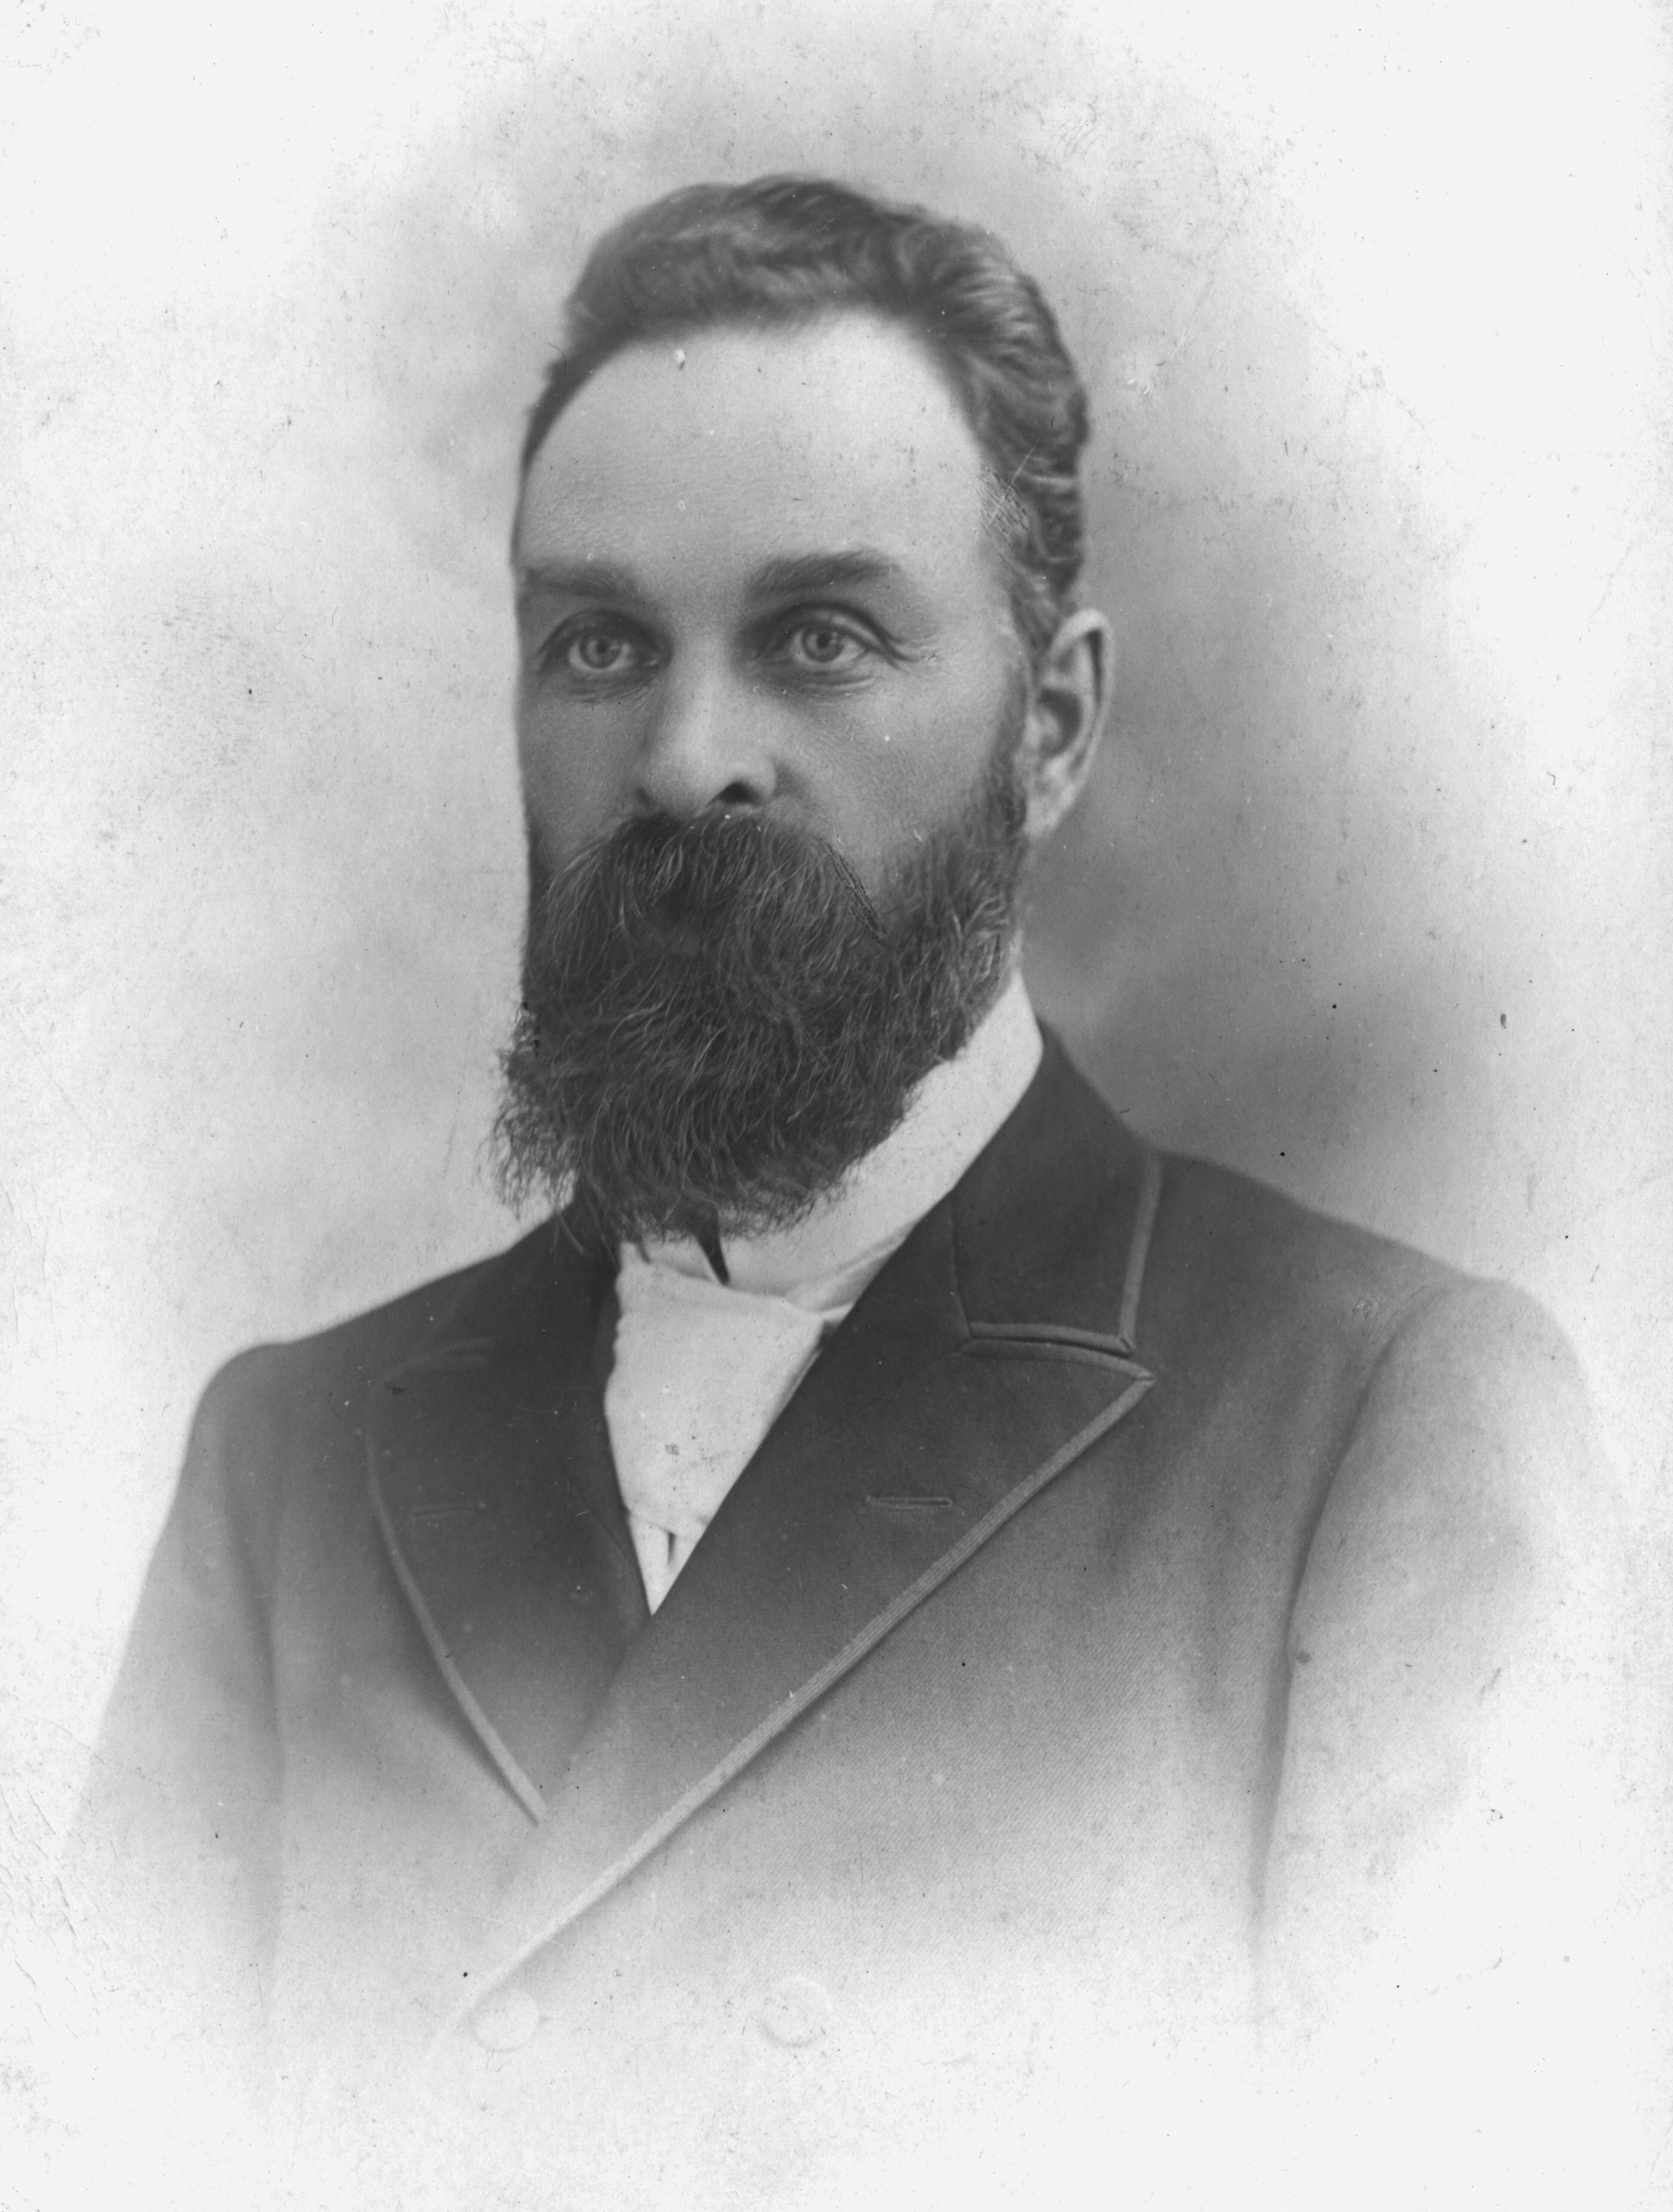
\includegraphics[width=1\linewidth]{images/daniels.jpg}
    \caption*{Arthur Grosvenor Daniells (1858-1935)}
    \label{fig:daniells}
\end{figure}


\begin{figure}[hp]
    \centering
    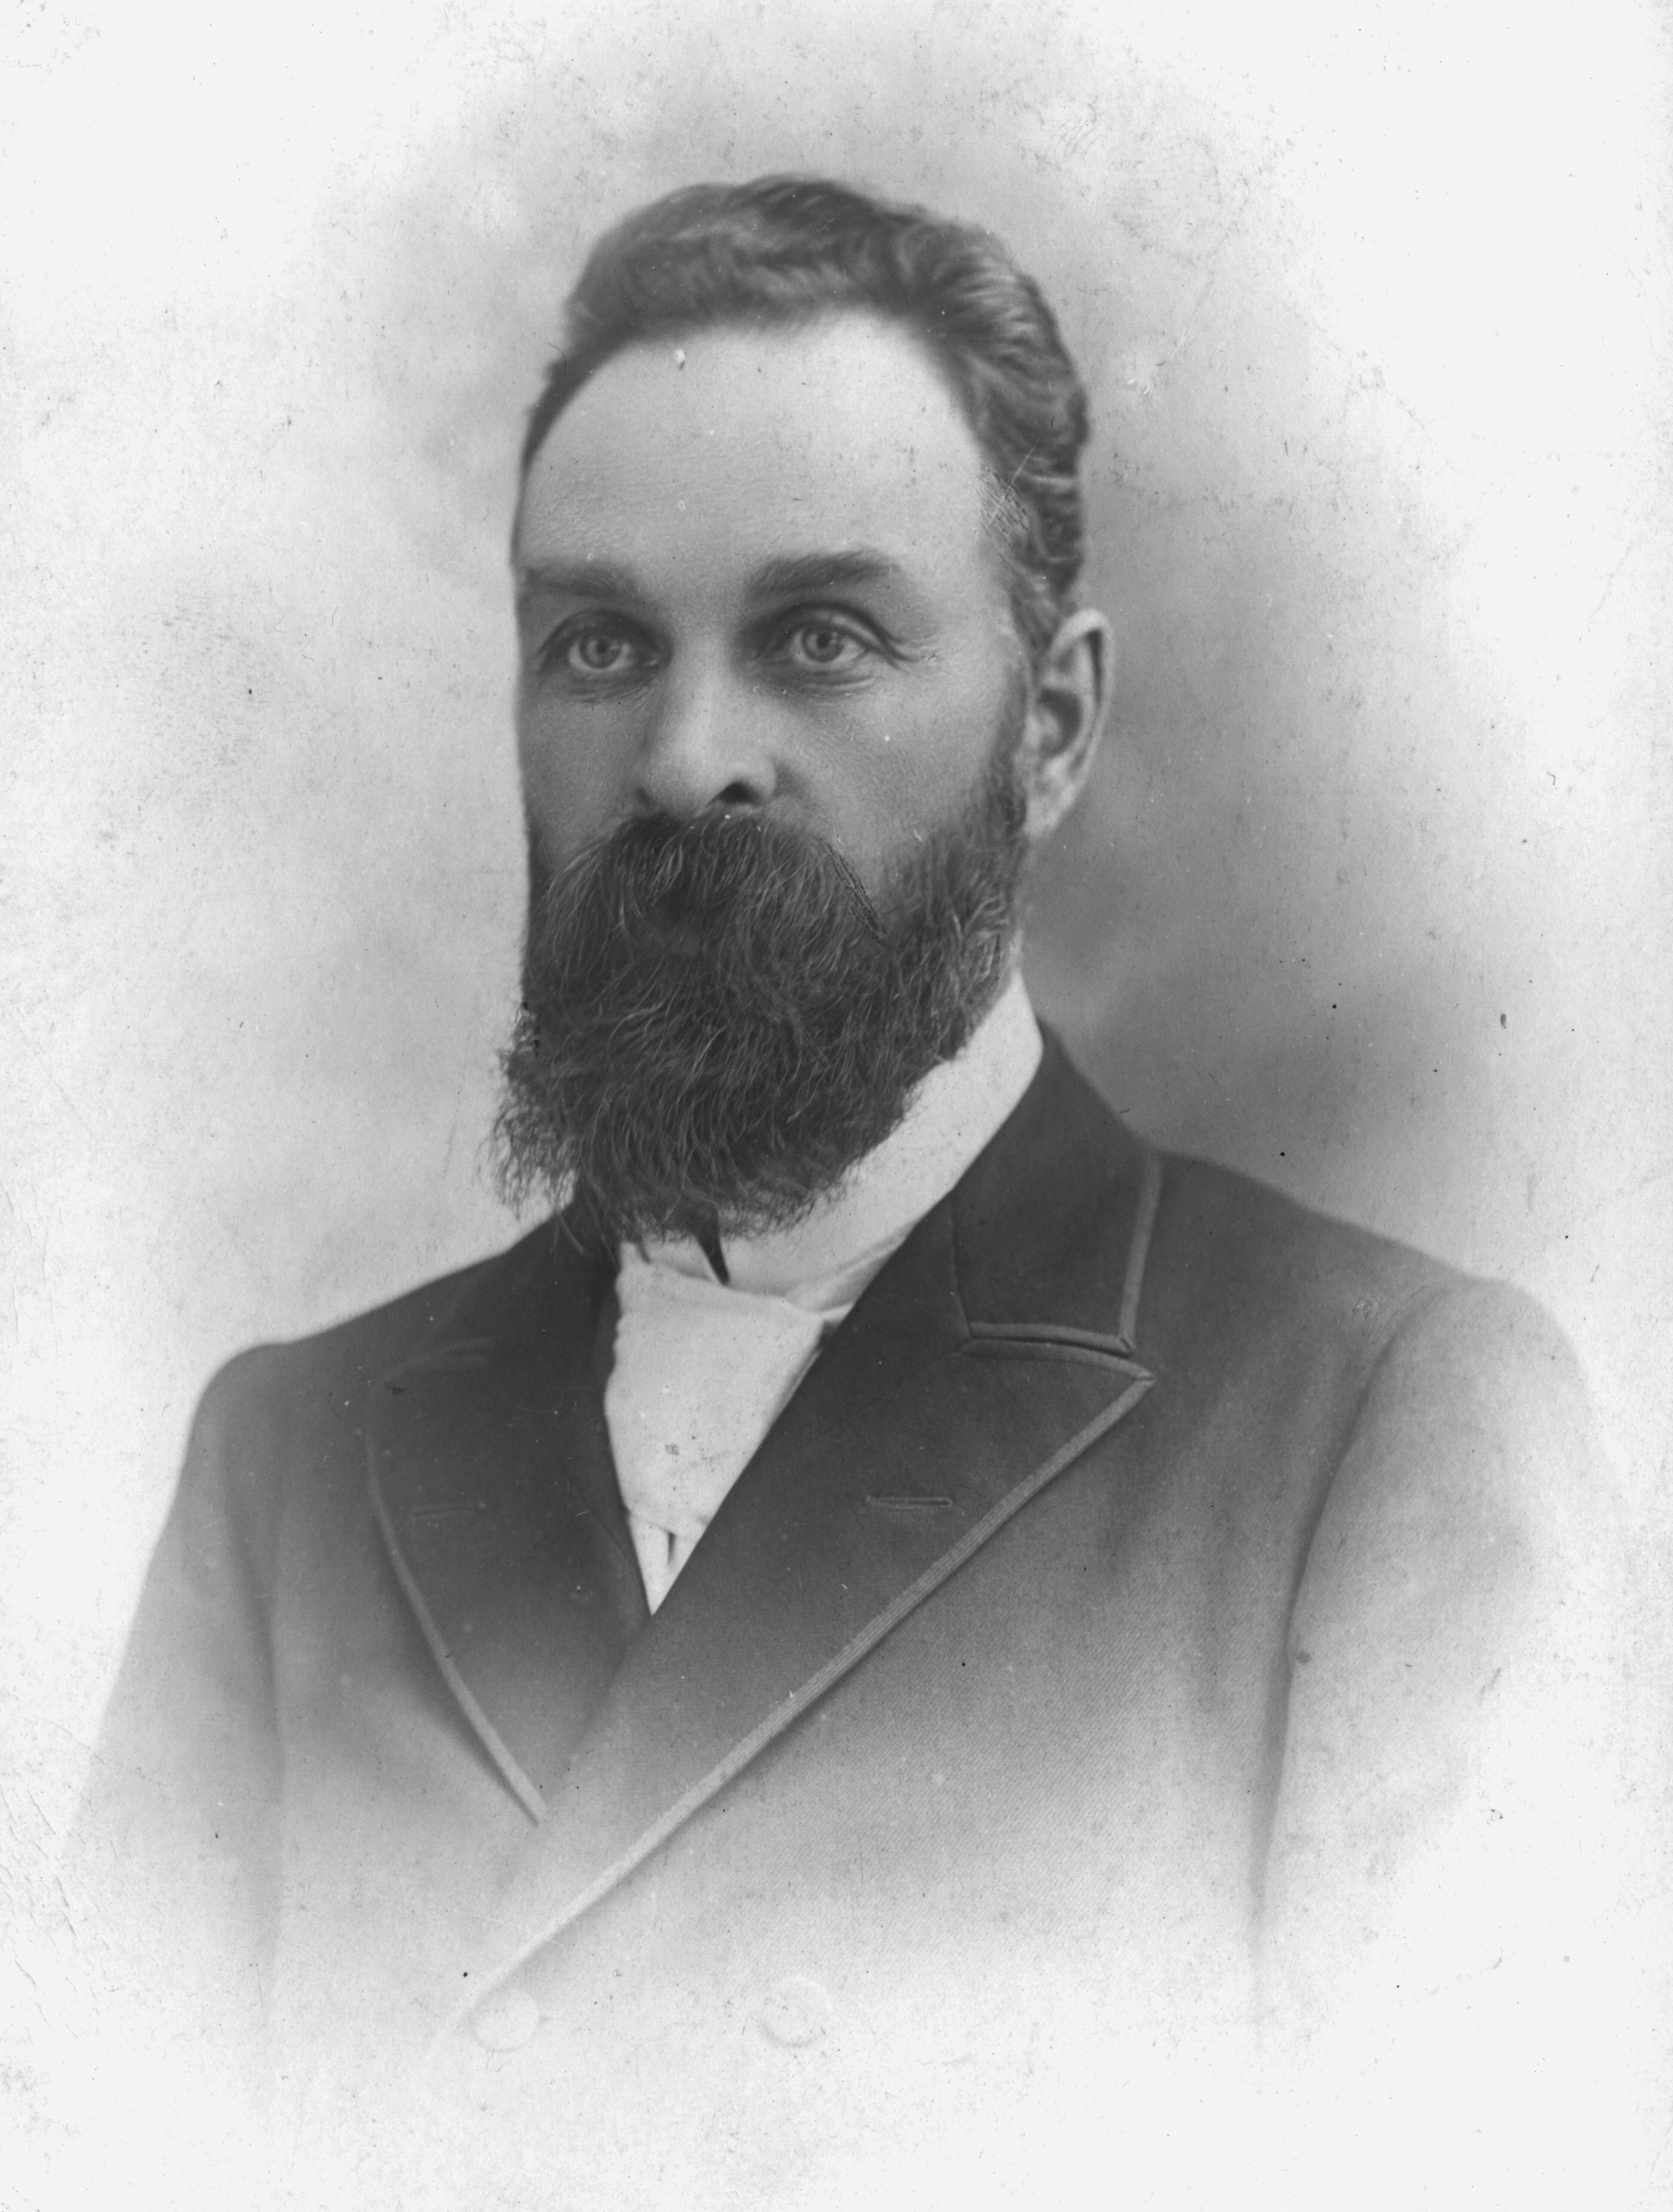
\includegraphics[width=1\linewidth]{images/daniels.jpg}
    \caption*{آرثر غروسفينور دانيلز (1858-1935)}
    \label{fig:daniells}
\end{figure}


\othersnogap{\textbf{He then stated that his former views \underline{regarding the trinity} had stood in his way of making a clear and absolutely correct statement; but that within a short time \underline{he had come to believe in the trinity} and could now see pretty clearly where all the difficulty was, and believed that he could clear the matter up satisfactorily.}}


\othersnogap{\textbf{ثم صرح أن آراءه السابقة \underline{بخصوص الثالوث} كانت عائقاً أمامه في تقديم بيان واضح وصحيح تماماً؛ لكنه خلال فترة قصيرة \underline{أصبح يؤمن بالثالوث} ويمكنه الآن أن يرى بوضوح أين كانت المشكلة، ويعتقد أنه يستطيع توضيح المسألة بشكل مُرضٍ.}}


\othersnogap{\textbf{He told me that he now believed in \underline{God the Father, God the Son, and God the Holy Ghost}; and his view was that it was God the Holy Ghost, and not God the Father, that filled all space, and every living thing. He said if he had believed \underline{this} before writing the book, he could have expressed his views without giving the wrong impression the book now gives.}}


\othersnogap{\textbf{أخبرني أنه يؤمن الآن \underline{بالله الآب، والله الابن، والله الروح القدس}؛ ورأيه هو أن الله الروح القدس، وليس الله الآب، هو الذي يملأ كل الفضاء وكل كائن حي. وقال إنه لو كان يؤمن \underline{بهذا} قبل كتابة الكتاب، لكان بإمكانه التعبير عن آرائه دون إعطاء الانطباع الخاطئ الذي يعطيه الكتاب الآن.}}


\othersnogap{\textbf{I placed before him the objections I found in the teaching, and tried to show him that the teaching was so utterly contrary to the gospel that I did not see how it could be revised by changing a few expressions.}}


\othersnogap{\textbf{عرضت أمامه الاعتراضات التي وجدتها في التعليم، وحاولت أن أبين له أن التعليم كان مخالفاً تماماً للإنجيل لدرجة أنني لم أر كيف يمكن تنقيحه بتغيير بعض التعبيرات.}}


\othersnogap{We argued the matter at some length in a friendly way; but I felt sure that when we parted, the doctor did not understand himself, nor the character of his teaching. And I could not see how it would be possible for him to flop over, \textbf{and in the course of a few days \underline{fix the books up} so that it would be all right}.}[Letter: A. G. Daniells to W. C. White, October 29, 1903. pp. 1, 2][https://forgotten-pillar.s3.us-east-2.amazonaws.com/Letter-A-G-Daniells-to-W-C-White-October-29-1903.pdf]


\othersnogap{ناقشنا المسألة لبعض الوقت بطريقة ودية؛ لكنني شعرت بالتأكيد أنه عندما افترقنا، لم يكن الطبيب يفهم نفسه، ولا طبيعة تعليمه. ولم أستطع أن أرى كيف سيكون من الممكن له أن يغير موقفه فجأة، \textbf{وفي غضون أيام قليلة \underline{يصلح الكتب} بحيث تصبح على ما يرام}.}[Letter: A. G. Daniells to W. C. White, October 29, 1903. pp. 1, 2][https://forgotten-pillar.s3.us-east-2.amazonaws.com/Letter-A-G-Daniells-to-W-C-White-October-29-1903.pdf]


Kellogg did not see the mistake in his sentiments; but rather, in expressing his views. He did not think that his views were false, merely his expression of those views, which led to the book giving a wrong impression. Yet, evidently, this was not true. As Sister White had stated, Kellogg had a problem with the sentiments regarding the \emcap{personality of God} and where His presence is. So, Kellogg suggested that in order to “\textit{fix the books up}” he would include the trinitarian expressions because he now started to believe in \textit{the Trinity} doctrine. At this point in time, the Seventh-day Adventist Church was not trinitarian—the doctrine of Trinity was not part of the \emcap{Fundamental Principles}, as we saw previously. Thus, it is no surprise that Brother Daniels objected and refuted Trinitarian teaching, claiming that it was\others{so utterly contrary to the gospel.} Revising the book, by changing a few expressions, would not change the main problem of the book: the sentiments on the \emcap{personality of God}.


لم يرَ كيلوغ الخطأ في آرائه؛ بل في التعبير عن وجهات نظره. لم يعتقد أن آراءه كانت خاطئة، بل مجرد تعبيره عن تلك الآراء، مما أدى إلى إعطاء الكتاب انطباعاً خاطئاً. ومع ذلك، من الواضح أن هذا لم يكن صحيحاً. كما ذكرت الأخت وايت، كان لدى كيلوغ مشكلة في الآراء المتعلقة بـ \emcap{شخصانية الله} وأين يوجد حضوره. لذلك، اقترح كيلوغ أنه من أجل “\textit{إصلاح الكتب}” سيضمن التعبيرات الثالوثية لأنه بدأ الآن يؤمن بعقيدة \textit{الثالوث}. في هذه النقطة الزمنية، لم تكن كنيسة الأدفنتست السبتيين ثالوثية—لم تكن عقيدة الثالوث جزءاً من \emcap{المبادئ الأساسية}، كما رأينا سابقاً. لذلك، ليس من المستغرب أن الأخ دانيلز اعترض ورفض التعليم الثالوثي، مدعياً أنه \others{مخالف تماماً للإنجيل.} إن تنقيح الكتاب، بتغيير بعض التعبيرات، لن يغير المشكلة الرئيسية للكتاب: الآراء حول \emcap{شخصانية الله}.


In the described events, and in William White's response to Brother Daniells, we can see why Sister White wrote the Special Testimonies. William White responded to Brother Daniells on Nov. 4, 1903:


في الأحداث الموصوفة، وفي رد ويليام وايت على الأخ دانيلز، يمكننا أن نرى لماذا كتبت الأخت وايت الشهادات الخاصة. رد ويليام وايت على الأخ دانيلز في 4 نوفمبر 1903:


\others{Dear Brother, --}


\others{أخي العزيز، --}


\othersnogap{\textbf{\underline{Mother and I} have just read your letter of \underline{October 29} in which you speak of the \underline{various plans that have been proposed for the revising and reproduction of ‘The Living Temple}.’}}


\othersnogap{\textbf{\underline{أمي وأنا} قرأنا للتو رسالتك المؤرخة في \underline{29 أكتوبر} التي تتحدث فيها عن \underline{الخطط المختلفة التي تم اقتراحها لمراجعة وإعادة إنتاج ‘ذا ليفينغ تمبل’}.}}


\othersnogap{We were pleasantly surprised at the announcement that Dr. Kellogg would withdraw this book from the market, \textbf{and we are sorry indeed that his mind is swinging back to the plan of revising it, \underline{Mother expresses herself quite emphatically regarding this matter; she regards it as an unprofitable undertaking}}. I think she will write to you soon expressing her views regarding this.}


\othersnogap{فوجئنا بشكل سار بالإعلان عن أن الدكتور كيلوغ سيسحب هذا الكتاب من السوق، \textbf{ونحن آسفون حقاً لأن عقله يعود إلى خطة تنقيحه، \underline{تعبر أمي عن نفسها بشكل حاسم للغاية بخصوص هذه المسألة؛ فهي تعتبرها مشروعاً غير مجدٍ}}. أعتقد أنها ستكتب إليك قريباً معبرة عن آرائها بخصوص هذا الأمر.}


\othersnogap{\textbf{… I believe it will be necessary \underline{to issue a special Testimony soon}, and this must contain a very full and clear statement on the positive side of this question, as well as articles pointing out the errors in the teaching of those who have departed from the truth through fascinating and deceptive theories}.}[\href{https://ellenwhite.org/letterbooks/555}{Letter from W.C. White to A.G. Daniells, Nov. 4, 1903,} (p. 458)]


\othersnogap{\textbf{... أعتقد أنه سيكون من الضروري \underline{إصدار شهادة خاصة قريبًا}، ويجب أن تحتوي هذه على بيان كامل وواضح جدًا عن الجانب الإيجابي من هذه المسألة، وكذلك مقالات تشير إلى الأخطاء في تعاليم أولئك الذين انحرفوا عن الحق من خلال نظريات فاتنة ومخادعة}.}[\href{https://ellenwhite.org/letterbooks/555}{رسالة من دبليو. سي. وايت إلى إيه. جي. دانيلز، 4 نوفمبر 1903،} (ص. 458)]


\begin{figure}[h]
    \centering
    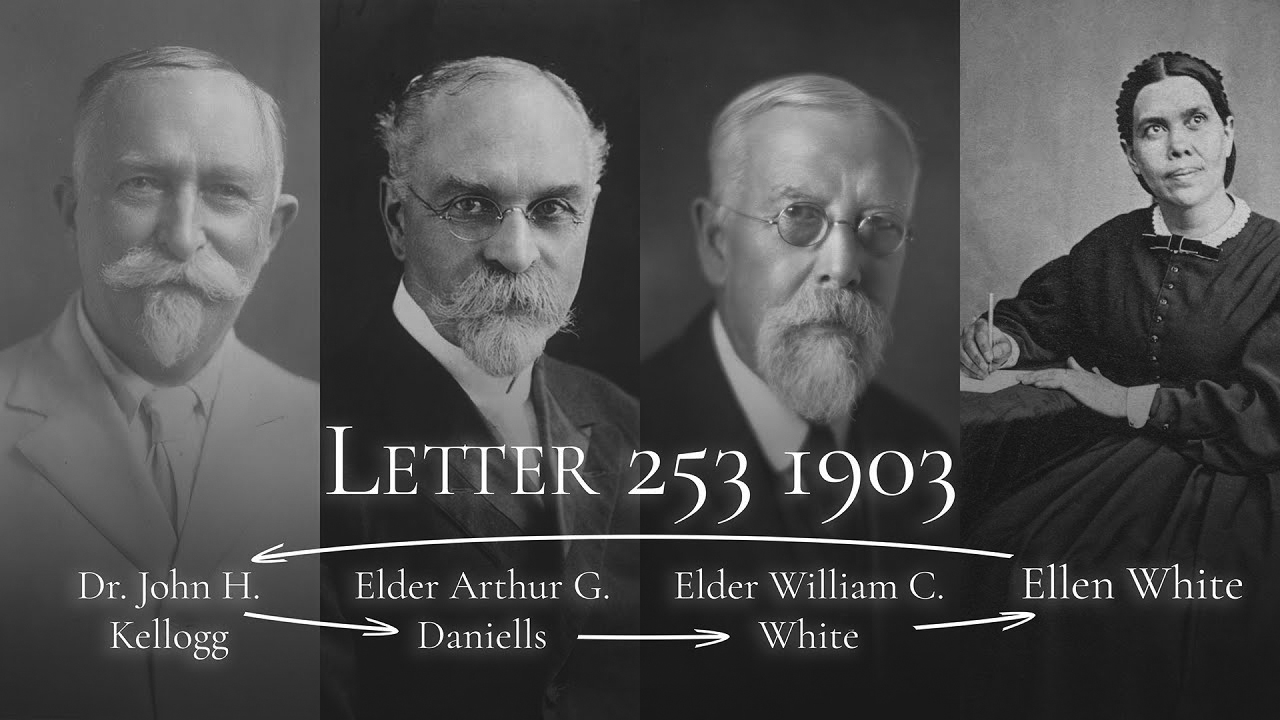
\includegraphics[width=1\linewidth]{images/correspondance.jpg}
    \caption*{Correspondence chain between A. G. Daniells, W. C. White, Ellen White and Dr. John H. Kellogg.}
    \label{fig:corespondance}
\end{figure}


\begin{figure}[h]
    \centering
    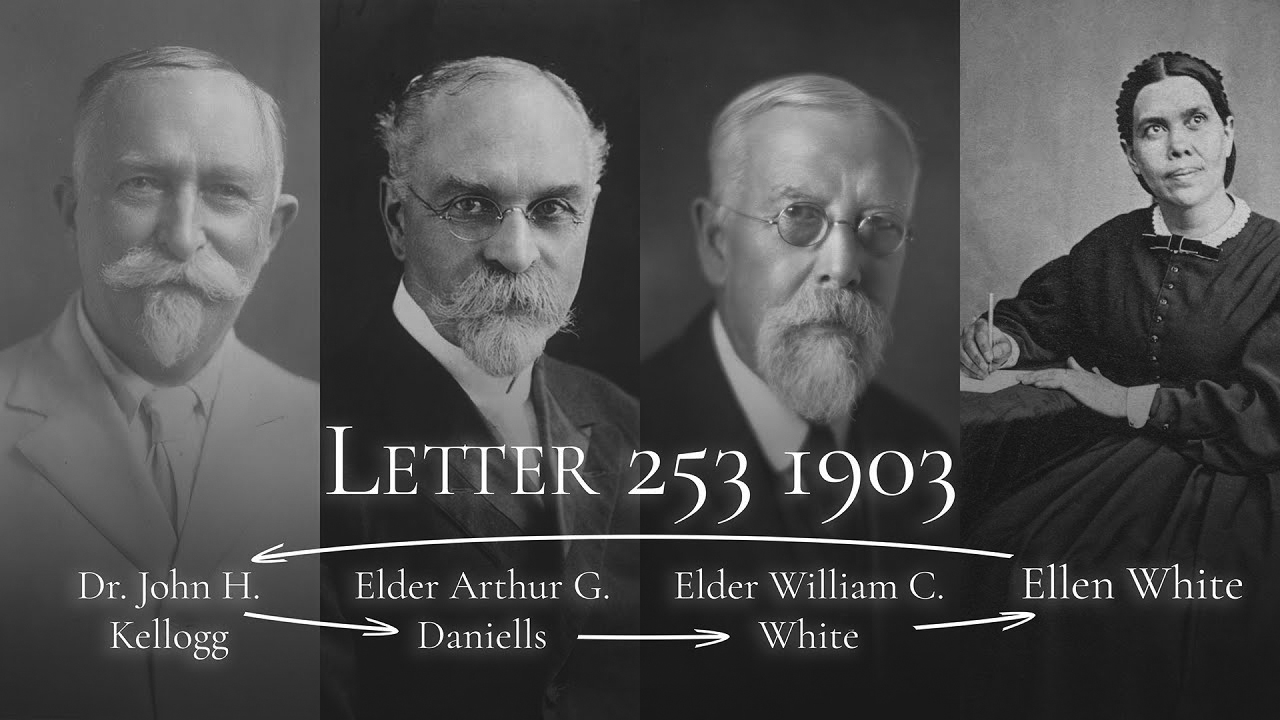
\includegraphics[width=1\linewidth]{images/correspondance.jpg}
    \caption*{سلسلة المراسلات بين إيه. جي. دانيلز، دبليو. سي. وايت، إلين وايت والدكتور جون إتش. كيلوغ.}
    \label{fig:corespondance}
\end{figure}


Here is evidence that Sister White was familiar with Dr. Kellogg's intentions to revise “\textit{Living Temple}” and her familiarity with his belief in the Trinity doctrine. In William's words, she expressed herself quite emphatically regarding this matter. She deemed it an unprofitable undertaking. For this reason, it was necessary to issue a special Testimony soon. And there it was. This is how the \textit{Testimonies for the Church Containing Letters to Physicians and Ministers Instruction to Seventh-Day Adventists} was published in 1904, containing letters to the physicians and ministers connected to Kellogg's crisis.


هنا دليل على أن الأخت وايت كانت على دراية بنوايا الدكتور كيلوغ لمراجعة “\textit{ذا ليفينغ تمبل}” ومعرفتها بإيمانه بعقيدة الثالوث. بكلمات ويليام، عبرت عن نفسها بشكل حاسم للغاية بخصوص هذه المسألة. اعتبرتها مسعى غير مجدٍ. لهذا السبب، كان من الضروري إصدار شهادة خاصة قريبًا. وها هي. هكذا تم نشر \textit{تستومنيز فور ذا شرش كنتاينينغ لترز تو فيزيشنز أند منسترز انستركشن تو سفنث داي أدفنتستس} في عام 1904، والتي تحتوي على رسائل إلى الأطباء والوزراء المرتبطين بأزمة كيلوغ.


By saying \others{\textbf{\underline{Mother and I} have just read your letter of \underline{October 29}}}, William testified that Sister White was fully aware of Kellogg's intentions and trinitarian belief. After she read Daniells’ letter, she wrote a direct reply to Dr. Kellogg. This letter is \textit{Lt253-1903}. It is a very prominent and eye opening letter because it clearly exposes how the prophet dealt with the Trinity doctrine. She elevated the doctrine on the \emcap{personality of God} constituted in the \emcap{Fundamental Principles}. There are striking similarities between this letter and the tenth chapter of the Special Testimonies, \textit{The Foundation of our Faith}.


بقوله \others{\textbf{\underline{قرأت أنا والوالدة} للتو رسالتك المؤرخة في \underline{29 أكتوبر}}، شهد ويليام أن الأخت وايت كانت على دراية تامة بنوايا كيلوغ ومعتقده الثالوثي. بعد أن قرأت رسالة دانيلز، كتبت ردًا مباشرًا إلى الدكتور كيلوغ. هذه الرسالة هي \textit{Lt253-1903}. إنها رسالة بارزة جدًا وتفتح العين لأنها تكشف بوضوح كيف تعاملت النبية مع عقيدة الثالوث. لقد رفعت من شأن عقيدة \emcap{شخصانية الله} المنصوص عليها في \emcap{المبادئ الأساسية}. هناك أوجه تشابه مذهلة بين هذه الرسالة والفصل العاشر من الشهادات الخاصة، \textit{أساس إيماننا}.


% Revision of the Living Temple

\begin{titledpoem}
    
    \stanza{
        In Kellogg’s book, a subtle snare \\
        Though well-disguised through crafty care \\
        From Bible truth would lead away \\
        And cause some precious souls to stray.
    }

    \stanza{
        And though much scripture there was used \\
        The early truth became confused \\
        This error served to twist the mind \\
        But in God’s Word the truth we find.
    }

    \stanza{
        God’s personality has form \\
        To Bible truth we must conform \\
        On this the Doctor wasn’t clear \\
        But early Advent truth is dear
    }
    
\end{titledpoem}